% Uso de la app: común a los manuales de Linux y de Windows (se incluye con \input)
% Antes de incluirlo, el manual define \abrirapp (cómo se abre la app en ese sistema).

% =====================================================================
\section{Seguridad}
\begin{itemize}
\item Mientras alguien tenga el mando del brazo real (en la PC o en un celular), una persona debe estar junto a la \textbf{seta de emergencia} del tablero. El paro de la página no la reemplaza.
\item El \textbf{selector del panel (I0.5)} decide quién manda: en \emph{manual} solo el panel; en \emph{automático} la PC o un operador remoto.
\item Con el brazo real, el mando desde la página está \textbf{deshabilitado} al empezar: hay que marcar una casilla y confirmar. Un solo operador tiene el mando a la vez.
\item Si la app, la página o el cable fallan, el PLC se detiene solo (watchdog de 2~s).
\item Antes de mover el brazo real, hacer siempre el \textbf{homing}.
\item Cada ingreso, cada orden aceptada y cada orden rechazada quedan en \codigo{registro\_gemelo.log}, con hora y usuario.
\end{itemize}

% =====================================================================
\section{El menú de inicio}\label{sec:menu}

Al abrir la app (\abrirapp) aparecen dos ventanas: una \textbf{consola} con los mensajes de la app y la \textbf{ventana del gemelo}, que empieza en el menú:

\begin{figure}[H]
\centering
\captura{\linewidth}{img/menu_inicio.jpg}{
  \node[marca] at (0.05,0.711) {1};
  \node[marca] at (0.05,0.533) {2};
  \node[marca] at (0.05,0.356) {3};
  \node[marca] at (0.05,0.272) {4};
  \node[marca] at (0.59,0.848) {5};
  \node[marca] at (0.59,0.565) {6};
  \node[marca] at (0.05,0.159) {7};
  \node[marca] at (0.905,0.959) {8};
}
\caption{Menú de inicio, con la simulación activa (la tarjeta del modo activo aparece resaltada y su botón dice \emph{Volver al gemelo}).}
\end{figure}
\begin{enumerate}[label=\num{\arabic*}, leftmargin=9mm]
\item \textbf{Simulación}: el brazo se mueve en pantalla con un PLC simulado dentro de la app. No necesita brazo ni cable.
\item \textbf{Operación local}: el gemelo sigue al brazo real y se lo puede mandar desde esta PC. Nadie más puede conectarse. La línea de abajo dice si se detecta el cable.
\item \textbf{Operación por red local}: como la operación local, y además celulares y otras PC de la misma red entran con usuario y contraseña.
\item \textbf{Sin brazo}: con esta casilla, la operación por red usa el PLC simulado; sirve para probar el acceso remoto sin la planta.
\item \textbf{Estado}: modo actual, conexión con el PLC, programa reconocido, quién tiene el mando y puertos serie detectados.
\item \textbf{Usuarios del acceso por red}: crear, cambiar el rol, cambiar la contraseña o quitar usuarios (sección \ref{sec:usuarios}).
\item \textbf{Ir al gemelo}: vuelve a la ventana del gemelo en el modo activo (aparece cuando ya hay un modo elegido).
\item Modo activo (al abrir la app por primera vez dice \emph{Sin modo}).
\end{enumerate}

\begin{center}\small
\begin{tabularx}{\linewidth}{>{\raggedright}p{3.2cm} >{\raggedright}X >{\raggedright}X >{\raggedright\arraybackslash}p{3.3cm}}
\toprule
\textbf{Modo} & \textbf{Para qué} & \textbf{Necesita} & \textbf{Quién se conecta}\\
\midrule
Simulación & aprender, practicar, preparar secuencias & nada & solo esta PC\\
Operación local & ver y mandar el brazo real desde la PC del laboratorio & cable USB-PPI, PLC en RUN & solo esta PC\\
Operación por red local & lo mismo, más supervisión y mando desde celulares & cable, al menos un usuario, misma red & esta PC y usuarios de la red\\
\bottomrule
\end{tabularx}
\end{center}

\textbf{Cambiar de modo.} En la barra superior del gemelo, el botón \textbf{«Menú»} (que muestra el modo activo) vuelve a este menú. Elegir otro modo cambia la conexión sin cerrar la app: al pasar de la simulación al brazo real se conecta con el PLC; al salir de la operación por red se cierra el acceso de los celulares. Al cambiar de modo se suelta el mando de los usuarios remotos.

\begin{figure}[H]
\centering
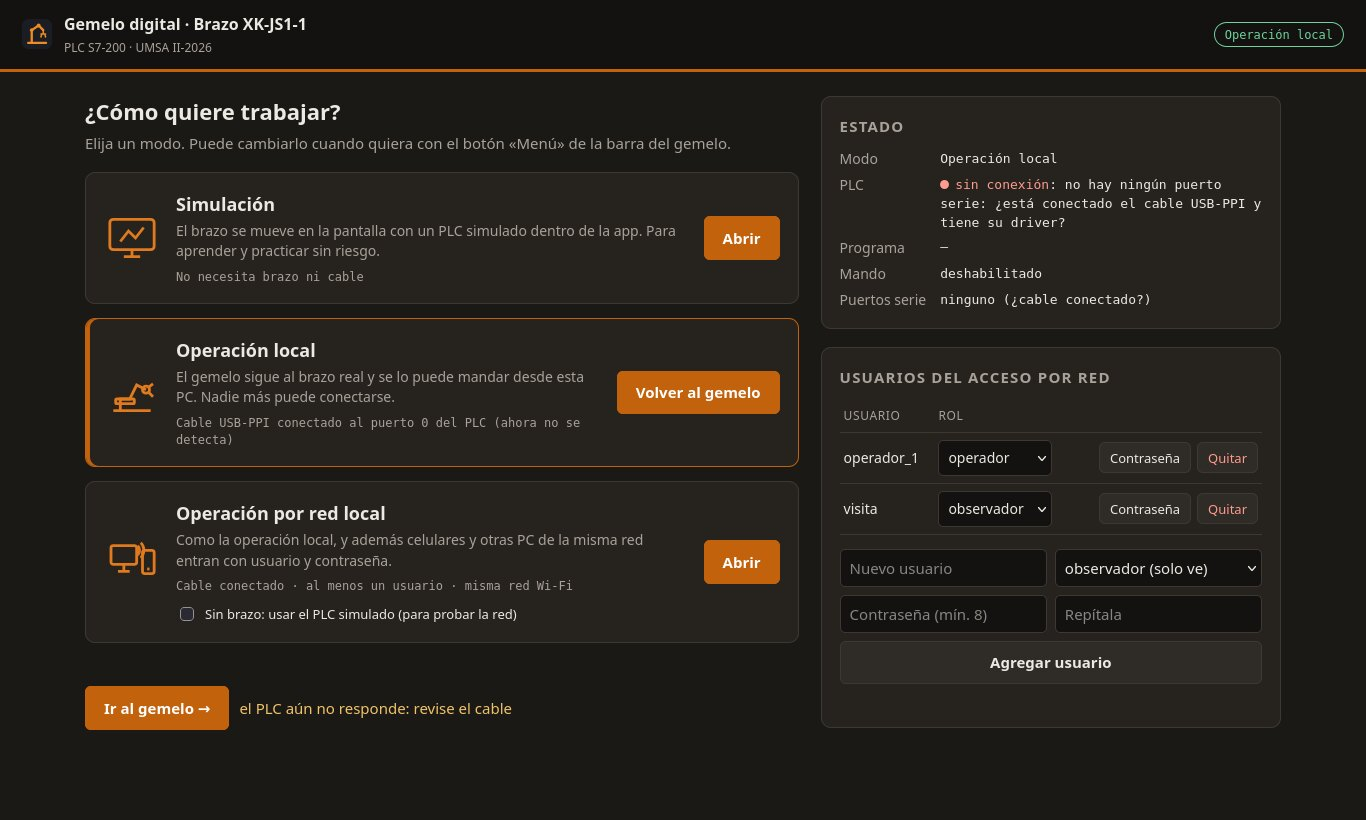
\includegraphics[width=0.92\linewidth]{img/menu_local_sin_cable.jpg}
\caption{Operación local elegida sin el cable conectado: el panel \emph{Estado} explica el motivo. La app sigue buscando el cable cada 2~s y se conecta sola al enchufarlo.}
\end{figure}

% =====================================================================
\section{La ventana del gemelo}\label{sec:gemelo}

La ventana es la misma en los tres modos. Las capturas están hechas en el modo simulación.

\begin{figure}[H]
\centering
\captura{\linewidth}{img/local_articular.jpg}{
  \node[marca] at (0.656,0.925) {1};
  \node[marca] at (0.86,0.925) {2};
  \node[marca] at (0.03,0.86) {3};
  \node[marca] at (0.61,0.855) {4};
  \node[marca] at (0.61,0.77) {5};
  \node[marca] at (0.61,0.505) {6};
  \node[marca] at (0.61,0.42) {7};
  \node[marca] at (0.012,0.094) {8};
  \node[marca] at (0.40,0.094) {9};
  \node[marca] at (0.012,0.048) {10};
}
\caption{Ventana del gemelo, pestaña \emph{Articular}.}
\end{figure}

\begin{enumerate}[label=\num{\arabic*}, leftmargin=9mm]
\item \textbf{Menú}: vuelve al menú de inicio; muestra el modo activo (solo en la PC del laboratorio).
\item \textbf{Estado de la conexión}: PLC conectado, programa reconocido (\emph{gemelo}) y quién tiene el mando.
\item \textbf{Visor 3D}: el brazo en la pose que informa el PLC. Se gira arrastrando con el ratón y se acerca con la rueda.
\item \textbf{Pestañas}: \emph{Articular}, \emph{Cartesiano}, \emph{Secuencias} y \emph{Conexión}.
\item \textbf{Ejes}: $\theta$ de la base, carro X y carro Y. Escriba el valor o suelte el deslizador donde quiera: el brazo va hasta ahí.
\item \textbf{Cerrar garra}, \textbf{Homing} y \textbf{Detener}.
\item \textbf{Velocidad de la simulación} y la casilla que imita el tren de pulsos compartido de X e Y (solo afecta a la simulación de la página).
\item \textbf{Vistas}: isométrica, frontal, lateral y superior.
\item \textbf{Espacio de trabajo} dibuja la zona alcanzable; \textbf{Trayectoria} deja la estela de la garra.
\item \textbf{Indicadores}: conexión, posición estimada, base sin calibrar, selector en manual, falta de homing, errores del PLC.
\end{enumerate}

\begin{figure}[H]
\centering
\captura{\linewidth}{img/local_conexion.jpg}{
  \node[marca] at (0.61,0.70) {1};
  \node[marca] at (0.61,0.58) {2};
  \node[marca] at (0.61,0.49) {3};
  \node[marca] at (0.61,0.43) {4};
  \node[marca] at (0.61,0.335) {5};
  \node[marca] at (0.61,0.245) {6};
}
\caption{Pestaña \emph{Conexión}.}
\end{figure}
\begin{enumerate}[label=\num{\arabic*}, leftmargin=9mm]
\item \textbf{Modo}: \emph{Brazo real (app del gemelo)} sigue a la app; \emph{Simulación} mueve solo el dibujo, sin la app.
\item \textbf{Leer estado}: vuelve a consultar la app.
\item \textbf{PLC y programa} reconocidos.
\item \textbf{Habilitar el mando}: con el brazo real hay que marcarla y confirmar para poder moverlo. En el modo simulación viene marcada.
\item \textbf{Pulsos}: velocidad de los motores, de 500 a 5000~Hz (a 4000~Hz los carros van a 20~mm/s). El programa no tiene rampas: conviene no pasar de 4000~Hz.
\item \textbf{Calibrar la base}: se escribe el ángulo medido con un transportador y la app calcula los pulsos por grado.
\end{enumerate}

\begin{figure}[H]
\centering
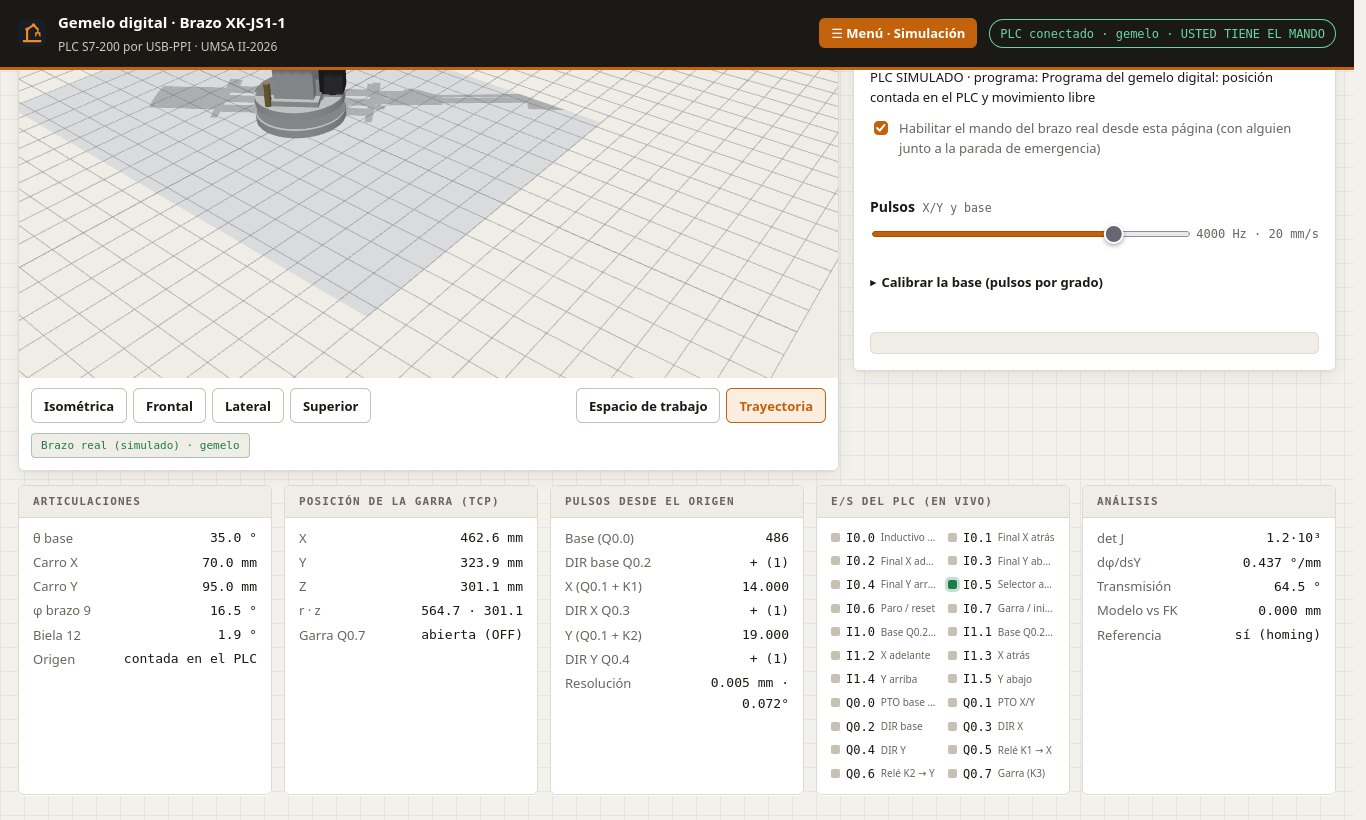
\includegraphics[width=\linewidth, trim=0 0 0 440, clip]{img/local_conexion_abajo.jpg}
\caption{Telemetría, debajo del visor: articulaciones, posición de la garra, pulsos desde el origen, entradas y salidas reales del PLC y análisis (jacobiano, transmisión, referencia).}
\end{figure}

\begin{figure}[H]
\centering
\captura{\linewidth}{img/local_cartesiano.jpg}{
  \node[marca] at (0.61,0.80) {1};
  \node[marca] at (0.61,0.66) {2};
  \node[marca] at (0.61,0.545) {3};
  \node[marca] at (0.61,0.47) {4};
}
\caption{Pestaña \emph{Cartesiano}, con un punto fuera del alcance.}
\end{figure}
\begin{enumerate}[label=\num{\arabic*}, leftmargin=9mm]
\item Origen en el eje de giro sobre la mesa; X apunta al sensor inductivo ($\theta = 0$) y Z hacia arriba.
\item \textbf{X, Y, Z} de la garra en mm.
\item \textbf{Mover} calcula la cinemática inversa y manda las posiciones de los ejes. \textbf{Usar posición actual} copia la posición de la garra en los campos.
\item Si el punto no se alcanza, la página propone el \textbf{punto alcanzable más cercano}; \emph{Usar ese punto} lo copia en los campos.
\end{enumerate}
\nota{\textbf{Por qué muchos puntos salen inalcanzables.} Los carros se mueven en diagonal y la garra solo alcanza una franja estrecha. Justo después del homing el brazo está en una esquina de esa franja: subir o bajar en vertical pide que el carro X retroceda por debajo de cero. Lo práctico es partir de \emph{Usar posición actual} y cambiar los valores de a poco.}

\begin{figure}[H]
\centering
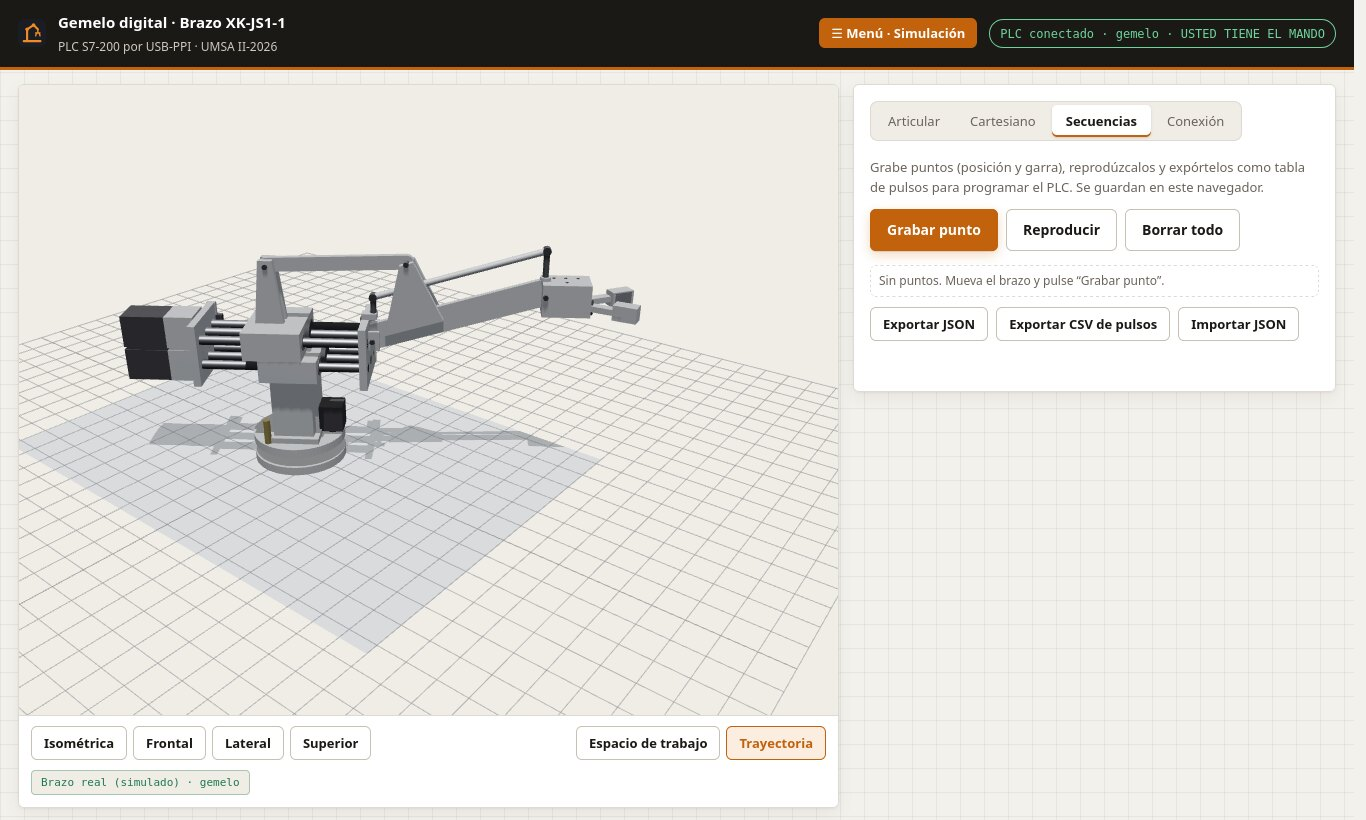
\includegraphics[width=0.9\linewidth]{img/local_secuencias.jpg}
\caption{Pestaña \emph{Secuencias}: \emph{Grabar punto} guarda la posición y la garra; \emph{Reproducir} los recorre esperando que el PLC termine cada uno; se exportan como JSON o como tabla CSV de pulsos.}
\end{figure}

\subsection{Primer uso con el brazo real}
\begin{enumerate}
\item En el menú, \textbf{Operación local} (o por red). Espere a que el estado diga \emph{PLC conectado}.
\item Selector del panel en \emph{automático}.
\item Pestaña \emph{Conexión}: marque \emph{Habilitar el mando} y confirme.
\item Pestaña \emph{Articular}: \textbf{Homing} (Y abajo, X atrás, abre la garra y gira la base al inductivo). Al terminar desaparece \emph{Sin referencia}.
\item Movimientos cortos primero (X 10~mm, Y 10~mm, $\theta$ 5°), comparando con una regla.
\end{enumerate}
Con el programa anterior del PLC (perfil \emph{cargado}) la página es sobre todo un monitor: la posición se estima y solo están las órdenes \emph{Iniciar}, \emph{Detener}, \emph{Paro de emergencia} y \emph{Rearmar}.

% =====================================================================
\section{Usuarios}\label{sec:usuarios}

La operación por red exige usuarios. Se administran en el menú de inicio, en el panel \emph{Usuarios del acceso por red}; solo se puede hacer desde la PC del laboratorio.

\begin{figure}[H]
\centering
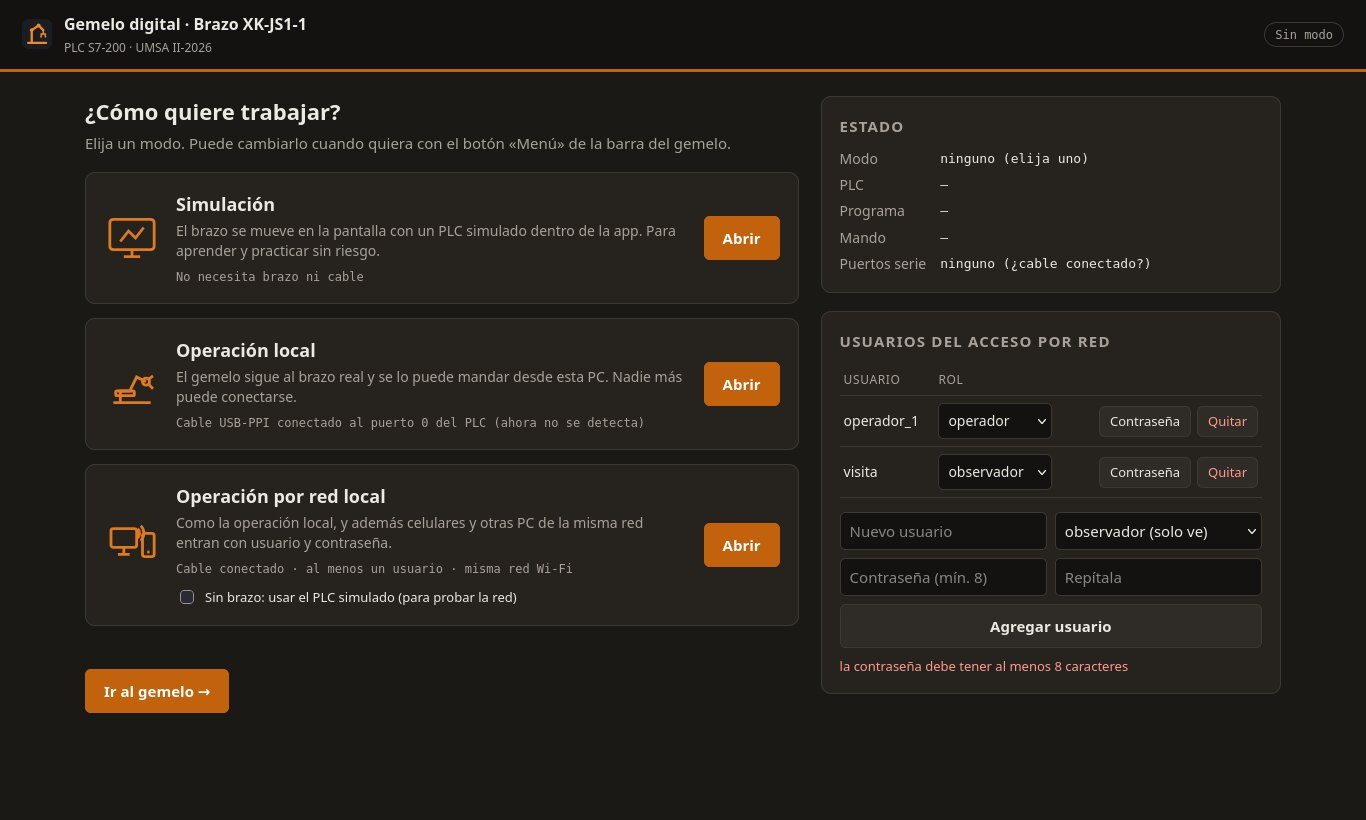
\includegraphics[width=0.92\linewidth]{img/menu_usuarios.jpg}
\caption{Panel de usuarios con dos usuarios creados. Al intentar crear uno con una contraseña corta, el menú lo rechaza y explica el motivo.}
\end{figure}

\begin{itemize}
\item \textbf{Agregar}: nombre (letras, números, punto, guion o guion bajo), rol y contraseña dos veces (al menos 8 caracteres).
\item \textbf{Rol}: el menú desplegable de cada fila lo cambia al momento.
\item \textbf{Contraseña}: pide la nueva dos veces. No hay forma de leer la anterior.
\item \textbf{Quitar}: pide confirmación; si ese usuario tenía el mando, lo pierde.
\end{itemize}

\begin{center}\small
\begin{tabularx}{\linewidth}{>{\raggedright}p{2.6cm} >{\raggedright\arraybackslash}X}
\toprule
\textbf{Rol} & \textbf{Qué puede hacer}\\
\midrule
observador & Ver el brazo en vivo: modelo 3D, posición, entradas y salidas. No puede mover, tomar el mando ni dar paro.\\
operador & Todo lo anterior, más tomar el mando y mover el brazo. Un solo operador tiene el mando a la vez; los demás ven quién lo tiene y pueden dar paro. El mando se suelta al desmarcar la casilla, al pulsar \emph{Salir} o tras 8~h sin uso.\\
\bottomrule
\end{tabularx}
\end{center}
Las contraseñas se guardan cifradas (PBKDF2) en \codigo{usuarios.json}, junto a la app. El nombre distingue mayúsculas. Tras 5 contraseñas erradas desde un equipo, ese equipo espera 60~s. Los usuarios también se pueden administrar desde una terminal con \codigo{usuarios.py} (\codigo{agregar}, \codigo{clave}, \codigo{rol}, \codigo{quitar}, \codigo{listar}).

% =====================================================================
\section{Operación por red local}\label{sec:red}

\begin{enumerate}
\item En el menú, \textbf{Operación por red local} (con la casilla \emph{Sin brazo} para probar con el PLC simulado). La primera vez la app crea el certificado del laboratorio; tarda unos segundos.
\item El panel \emph{Estado} muestra la dirección para los celulares, con un botón \emph{Copiar}:
\end{enumerate}

\begin{figure}[H]
\centering
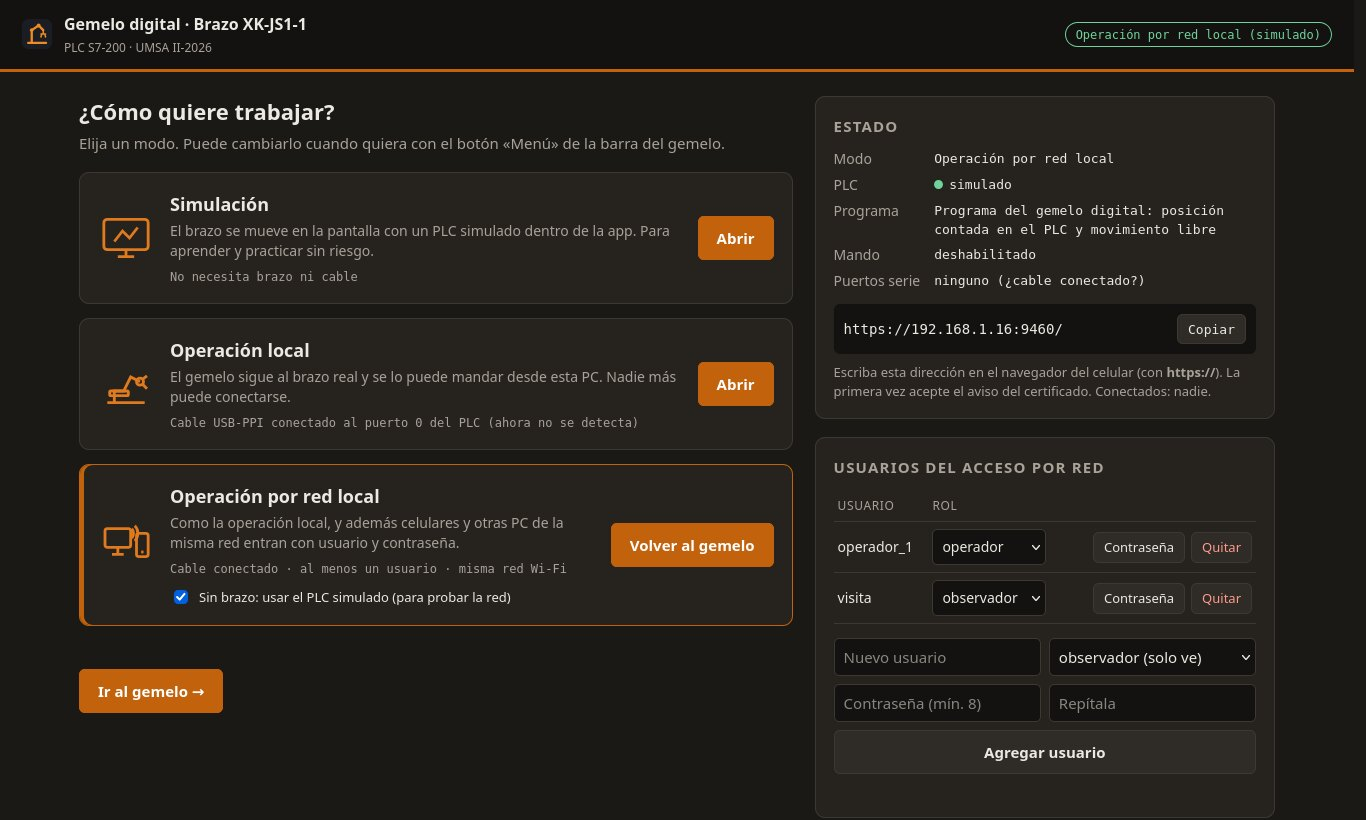
\includegraphics[width=0.92\linewidth]{img/menu_red.jpg}
\caption{Operación por red local activa: la dirección \texttt{https://IP:8443/} y quiénes están conectados.}
\end{figure}

\begin{enumerate}[resume]
\item Conecte el celular \textbf{al mismo Wi-Fi o router} que la PC del laboratorio (con datos móviles no funciona).
\item Escriba la dirección \textbf{con \codigo{https://} y con el puerto \codigo{:8443}}. La primera vez el navegador avisa que la conexión no es privada: el certificado es propio del laboratorio. Pulse \emph{Avanzado $\rightarrow$ Continuar}.
\item Ingrese con su usuario y contraseña.
\end{enumerate}

\begin{figure}[H]
\centering
\begin{minipage}[t]{0.31\linewidth}\centering
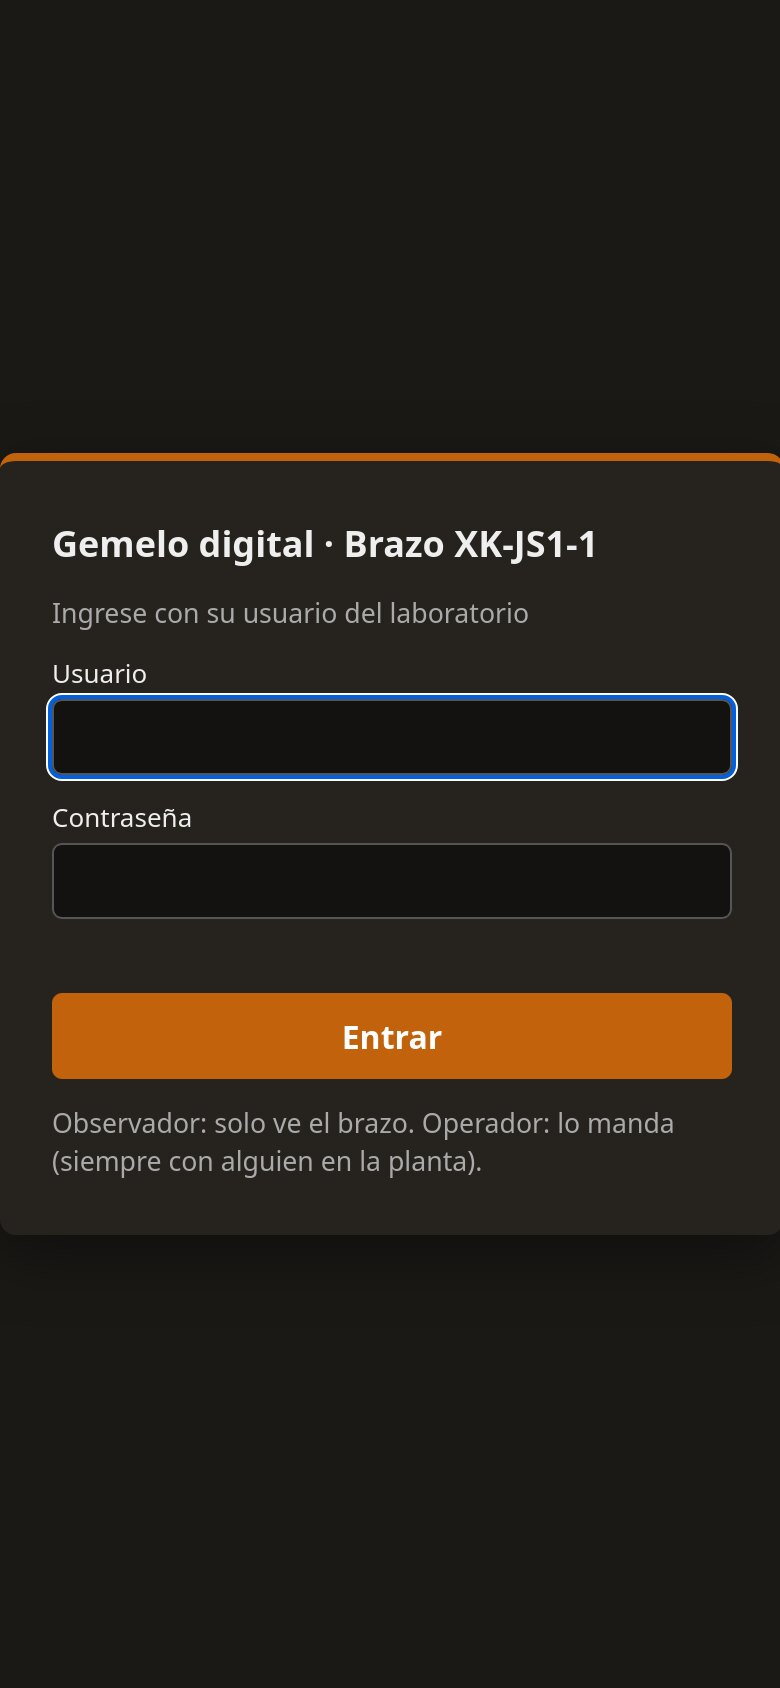
\includegraphics[width=\linewidth]{img/remoto_login.jpg}\\[2pt]{\small (a) ingreso}
\end{minipage}\hfill
\begin{minipage}[t]{0.31\linewidth}\centering
\captura{\linewidth}{img/remoto_observador.jpg}{
  \node[marca] at (0.80,0.955) {1};
  \node[marca] at (0.50,0.905) {2};
  \node[marca] at (0.07,0.03) {3};
}\\[2pt]{\small (b) observador}
\end{minipage}\hfill
\begin{minipage}[t]{0.31\linewidth}\centering
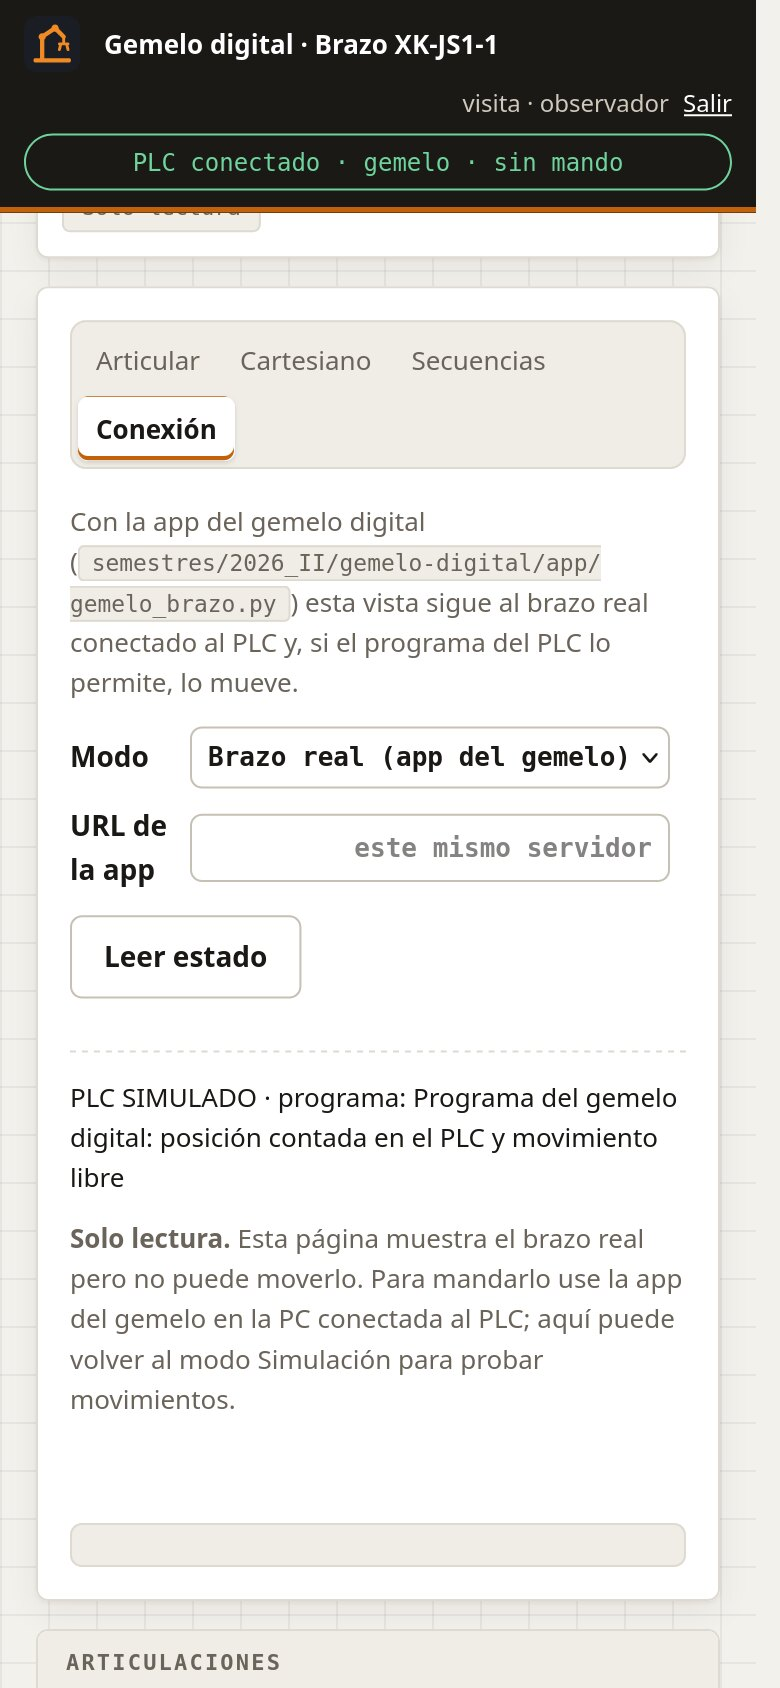
\includegraphics[width=\linewidth]{img/remoto_observador_conexion.jpg}\\[2pt]{\small (c) observador, Conexión}
\end{minipage}
\caption{Acceso remoto desde un celular como \textbf{observador}.}
\end{figure}
\begin{enumerate}[label=\num{\arabic*}, leftmargin=9mm]
\item Usuario y rol, y \emph{Salir} para cerrar la sesión. Desde la red no aparece el botón «Menú»: el modo solo se cambia en la PC del laboratorio.
\item Estado: PLC conectado, programa y quién tiene el mando.
\item \emph{Solo lectura}: los controles aparecen bloqueados. Si igual intenta mandar, la app lo rechaza y lo anota en el registro.
\end{enumerate}

\begin{figure}[H]
\centering
\begin{minipage}[t]{0.31\linewidth}\centering
\captura{\linewidth}{img/remoto_operador_conexion_antes.jpg}{\node[marca] at (0.05,0.34) {1};}\\[2pt]{\small (a) operador, sin mando}
\end{minipage}\hfill
\begin{minipage}[t]{0.31\linewidth}\centering
\captura{\linewidth}{img/remoto_operador_conexion.jpg}{\node[marca] at (0.06,0.905) {2}; \node[marca] at (0.05,0.40) {3};}\\[2pt]{\small (b) mando tomado}
\end{minipage}\hfill
\begin{minipage}[t]{0.31\linewidth}\centering
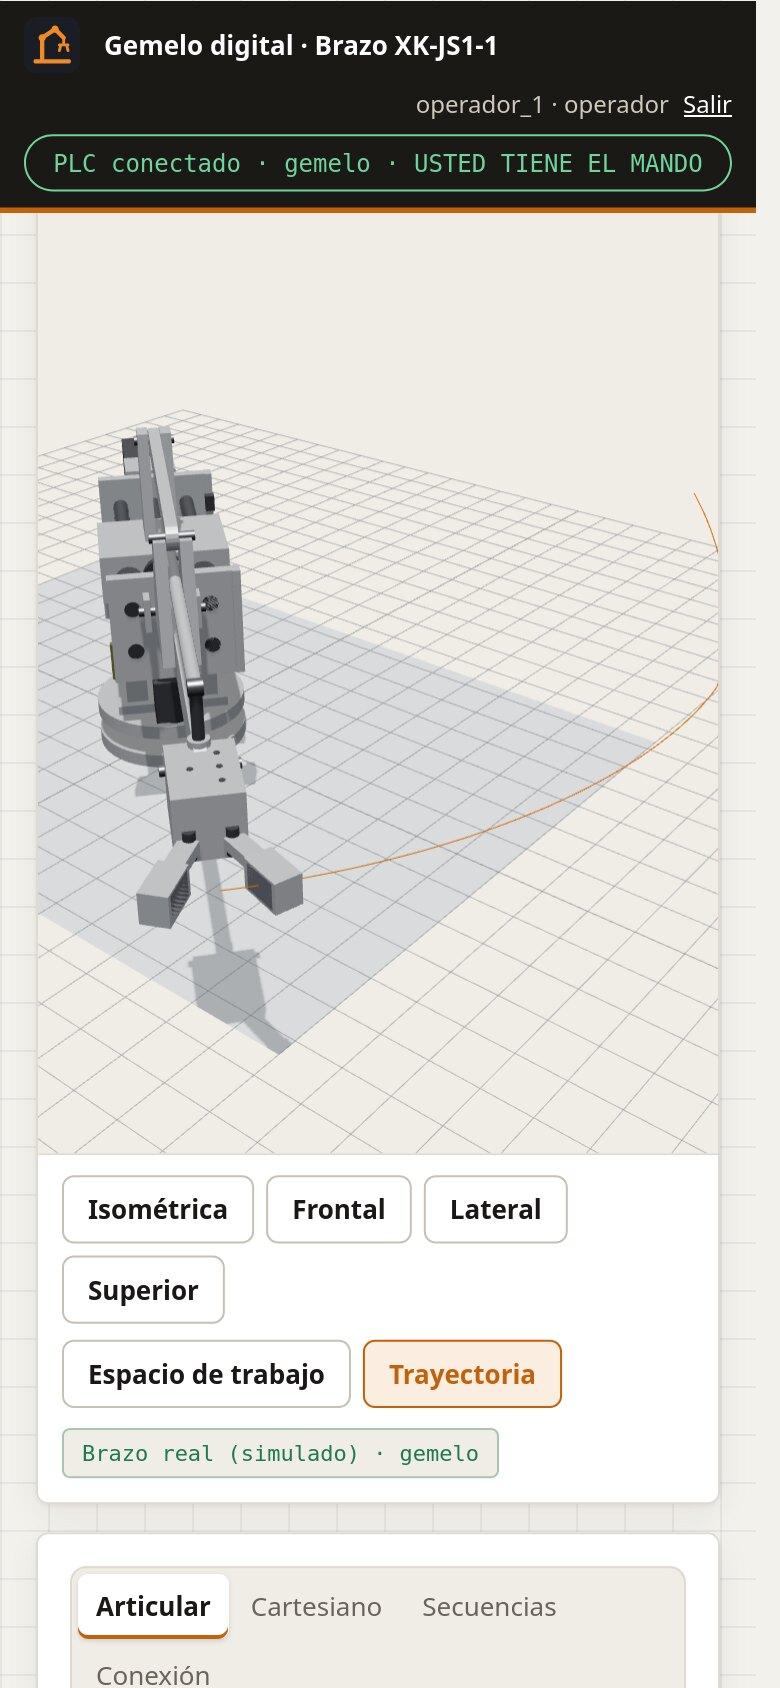
\includegraphics[width=\linewidth]{img/remoto_operador_mueve.jpg}\\[2pt]{\small (c) el brazo se movió}
\end{minipage}
\caption{Acceso remoto como \textbf{operador}.}
\end{figure}
\begin{enumerate}[label=\num{\arabic*}, leftmargin=9mm]
\item Al ingresar, el operador no tiene el mando: la casilla \emph{Habilitar el mando} está vacía.
\item Al marcarla y confirmar, el estado pasa a \emph{USTED TIENE EL MANDO}.
\item Desde ahí usa las pestañas igual que en la PC del laboratorio (sección \ref{sec:gemelo}).
\end{enumerate}

\nota{\textbf{La app debe estar abierta en la PC del laboratorio} mientras se use el brazo desde los celulares: es la única que habla con el PLC. Si se cierra, los celulares ven \emph{Sin conexión} y el PLC detiene cualquier movimiento en curso. El acceso llega solo a la red local; para usarlo desde internet haría falta una VPN.}

\subsection{Comprobar qué hace cada usuario}
La consola de la app y el archivo \codigo{registro\_gemelo.log} muestran los ingresos y las órdenes:
\begin{lstlisting}
00:59:50 modo: Operación por red local
00:59:55 ingreso de visita (observador) desde 192.168.1.20
01:00:12 RECHAZADO /api/orden/mover de visita (observador): solo puede ver
01:00:20 ingreso de operador_1 (operador) desde 192.168.1.9
01:00:25 mando desde la PC HABILITADO (operador_1)
01:00:31 orden homing  (operador_1)
\end{lstlisting}

% =====================================================================
\section{La página pública}
La página publicada en internet (\url{https://brazo-4gdl-gemelo-digital.pages.dev}) sirve para estudiar y simular el brazo. Abierta en la propia PC del laboratorio, con la app en marcha, puede además \emph{ver} el brazo real (pestaña \emph{Conexión}, modo \emph{Brazo real}, URL \codigo{http://localhost:8050}), pero nunca mandarlo.

% =====================================================================
\section{Solución de problemas comunes}
\begin{center}\small
\begin{longtable}{>{\raggedright}p{5.4cm} >{\raggedright\arraybackslash}p{10.4cm}}
\toprule
\textbf{Síntoma} & \textbf{Qué hacer}\\
\midrule
\endhead
Estado: \emph{no hay ningún puerto serie} & El cable no está enchufado o le falta el driver.\\
Estado: \emph{no responde ningún PLC} & PLC apagado o en STOP, cable fuera del puerto 0, o Micro/WIN tiene el puerto abierto.\\
\emph{para la operación por red cree antes al menos un usuario} & Cree un usuario en el panel \emph{Usuarios} del menú.\\
\emph{no se pudo abrir el acceso por red} & Otro programa usa el puerto 8443 (por ejemplo, otra copia de la app abierta). Ciérrela.\\
El celular no abre la página & Use \codigo{https://} y \codigo{:8443}; mismo Wi-Fi; revise el cortafuegos (sección de instalación). Redes de invitados pueden aislar a los equipos.\\
\emph{La conexión no es privada} & Normal la primera vez: \emph{Avanzado $\rightarrow$ Continuar}.\\
\emph{Usuario o contraseña incorrectos} & El nombre distingue mayúsculas. Cambie la contraseña desde el menú.\\
\emph{su usuario es observador} & Ese usuario solo puede ver: cambie su rol a operador en el menú.\\
\emph{Mando en uso por \dots} & Otro operador tiene el mando: puede dar paro, pero no mover hasta que lo suelte.\\
\emph{el mando desde la PC está deshabilitado} & Marque \emph{Habilitar el mando} en la pestaña \emph{Conexión}.\\
\emph{Selector en manual} & Gire el selector del panel a automático.\\
\emph{falta hacer homing} & Use \emph{Homing}.\\
\emph{Inalcanzable} en \emph{Cartesiano} & Use \emph{Usar ese punto} o cambie los valores de a poco.\\
\emph{watchdog} & La página o la app dejaron de responder durante un movimiento: vuelva a hacer homing.\\
El modelo no coincide con el brazo & Haga homing.\\
\bottomrule
\end{longtable}
\end{center}
